\documentclass[aspectratio=169, usenames, dvipsnames]{beamer}

\usepackage{xcolor}
\usepackage[normalem]{ulem} % for strikethrough text

% set up minted
\usepackage{minted}
\setminted{autogobble=true, linenos=false, fontsize=\footnotesize}
\usemintedstyle{friendly}

\definecolor{rustcolor}{rgb}{0.95,0.95,0.95}

% LAST import: menukeys
\usepackage{menukeys}
\renewmenumacro{\menu}[>]{roundedmenus}

% for semi transparent text
\newcommand{\semitransp}[2][35]{\textcolor{fg!#1}{#2}}

% setup for footnotes...
\addtobeamertemplate{footnote}{\vspace{-8pt}\advance\hsize-0.5cm}{\vspace{8pt}}
\makeatletter
\renewcommand*{\footnoterule}{\kern -3pt \hrule \@width 2in \kern 10.6pt}
\setbeamerfont{footnote}{size=\tiny}

\title{Ohua as STM alternative for shared state applications}
\subtitle{Master Midway Defense}
\date{29. January 2020}
\author{Felix Wittwer}

\usetheme{ccc}

\begin{document}

\begin{frame}
\titlepage
\end{frame}

\begin{frame}{Ohua\footnotemark[1]}
  \begin{columns}
    \begin{column}{0.7\textwidth}
      Framework for implicit parallel programming:\\[.55\baselineskip]
      \begin{itemize}
        \item<2-> Derives dataflow graph from algorithm file
        \item<3-> Runs optimizations on graph to exploit parallelism at compile time
        \item<4-> Generates native runtime code
      \end{itemize}
      % TODO: Zusätzlichen Punkt, der Ohua besser verkauft für dieses Problem.
    \end{column}
    \begin{column}{0.25\textwidth}
      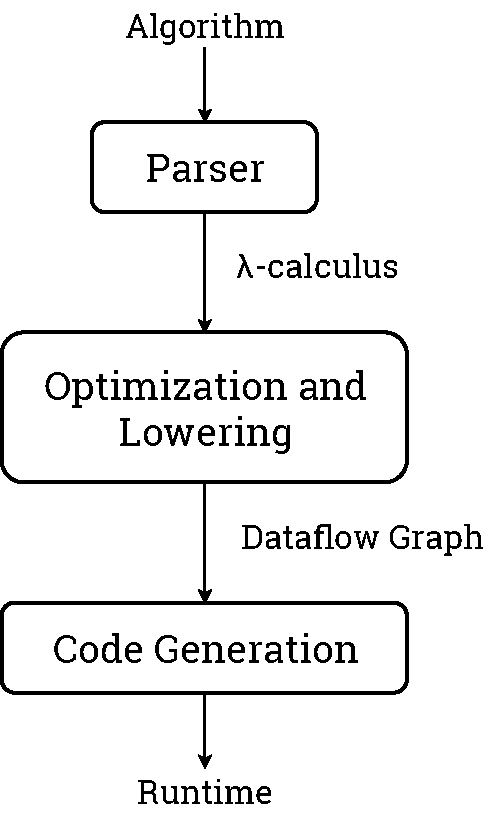
\includegraphics[width=\textwidth,height=\textheight,keepaspectratio]{img/ohua}
    \end{column}
  \end{columns}
  % TODO: Chart showing what it does (?), bullet point that we want to make a comparison
  % \vfill

  % \uncover<4->{\textbf{Challenges:}}
  % \begin{itemize}
  % \item<4->{Ohua does not provide primitives for transactions}
  %   \begin{itemize}
  %   \item<5-> Use \texttt{smap} and shared state
  %   \end{itemize}
  % \item<6-> Problem: Collision handling
  %   \begin{itemize}
  %   \item<7-> Collect failed jobs and call transaction recursively
  %   \end{itemize}
  % \end{itemize}
  \footnotetext[1]{Ertel et al. "Towards Implicit Parallel Programming for Systems." dissertation, 2019.}
\end{frame}

\begin{frame}{Throwback: Labyrinth Benchmark}
  \begin{columns}
    \begin{column}{0.5\textwidth}
      \textbf{Given:} 3D maze, pairs of points\\[\baselineskip]

      \uncover<2->{\textbf{Goal:} Map a path between each pair of points\\[\baselineskip]}

      \uncover<3->{\textbf{Implementation:}}
      \begin{itemize}
      \item<3-> parallel search for new paths
      \item<4-> merge paths into the maze\\\uncover<5->{$\rightarrow$ retry if path crosses other paths}
      \end{itemize}
    \end{column}
    \begin{column}{0.5\textwidth}
      \begin{center}
        \includegraphics<1-2>[width=.9\textwidth]{img/1-maze_points}%
        \includegraphics<3>[width=.9\textwidth]{img/2-maze_paths}%
        \includegraphics<4>[width=.9\textwidth]{img/4-maze_update2}%
        \includegraphics<5->[width=.9\textwidth]{img/5-maze_update3}%
      \end{center}
    \end{column}
  \end{columns}
\end{frame}

% TODO: basically the old graphs with the bad performance
\begin{frame}{Throwback: Early Results}
  \begin{columns}
    \begin{column}{0.55\textwidth}
      \centering
      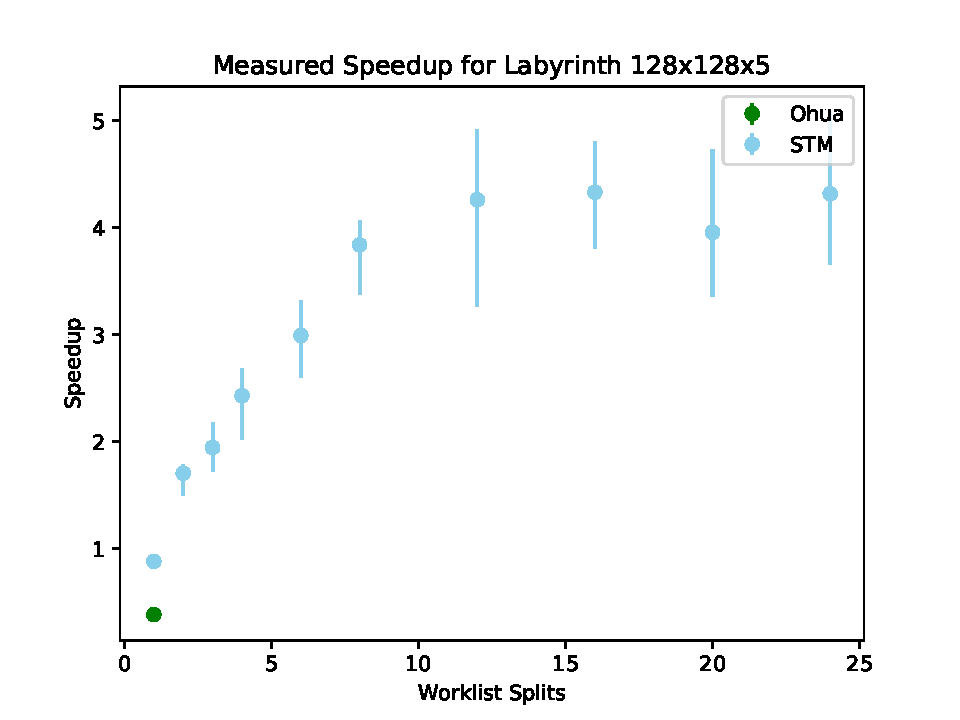
\includegraphics[width=\textwidth,height=.7\textheight,keepaspectratio]{img/2019-04-18-128x128x5}
    \end{column}
    \begin{column}{0.45\textwidth}
      \begin{itemize}
        \item Ohua: one measuring point
        \item Speedup < 0.5
        \item<2-> Bad resource usage
        \item<2-> No configurable threadpool size
      \end{itemize}
    \end{column}
  \end{columns}
\end{frame}

\begin{frame}{Improving the Benchmark Performance}
  \textbf{Previousy envisioned steps:}\\

  \begin{enumerate}
    % TODO: Maybe uncover one by one
    \item \only<1-1>{add a simple scheduler to the runtime to improve measurability}\only<2->{\semitransp{\sout{add a simple scheduler to the runtime to improve measurability}}}
    \item<3-> implement data parallelism \only<1-3>{in \texttt{smap} operator}\only<4->{\semitransp{\sout{in \texttt{smap} operator}} manually}\\[.55\baselineskip]
    \item<5-> reduce the number of retries by moving the state updates
      \begin{itemize}
      \item<5-> \only<1-5>{requires thinking about how state sharing should work}\only<6->{\semitransp{\sout{requires thinking about how state sharing should work}}}\\[.55\baselineskip]
      \end{itemize}
  \end{enumerate}

  \vspace{2em}

  \uncover<7->{\textbf{Goal:} Finding generalized dataflow transformations}\\
  \hspace*{1cm} \uncover<8->{$\rightarrow$ develop proof of concept implementations}
\end{frame}

\begin{frame}{Transformation 1: Worklist Splits}
  \begin{columns}
    \begin{column}{.5\textwidth}
      \inputminted[bgcolor=rustcolor, fontsize=\tiny]{rust}{code/initial.rs}
    \end{column}
    \begin{column}{.5\textwidth}
      \uncover<3->{\inputminted[bgcolor=rustcolor, fontsize=\tiny]{rust}{code/split.rs}}
    \end{column}
  \end{columns}
  
  \begin{itemize}
    \item<2-> Split worklist into $m$ equally large parts and run path-finding data-parallel
  \end{itemize}
  \vfill
\end{frame}

\begin{frame}{Transformation 1: Worklist Splits}
  \begin{columns}
    \begin{column}{0.45\textwidth}
      \begin{itemize}
        \item<3-> Granular parallelism control
        \item<4-> Still only about half the speedup \alert{\texttt{stm}} shows
      \end{itemize}

      \vspace{1.5em}
      \uncover<5->{\textbf{Reason:} Straggler Problem}
      \begin{itemize}
        \item<6-> Synchronization points force all threads to wait
      \end{itemize}
    \end{column}
    \begin{column}{0.55\textwidth}
      \centering%
      \only<1>{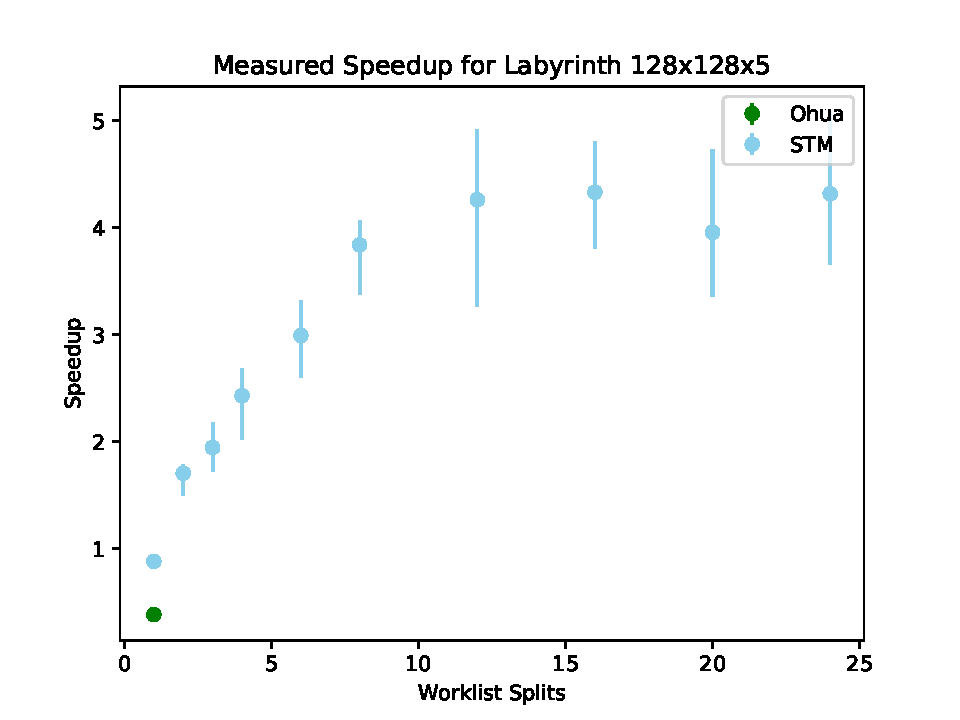
\includegraphics[width=\textwidth,height=.7\textheight,keepaspectratio]{img/2019-04-18-128x128x5}}%
      \only<2->{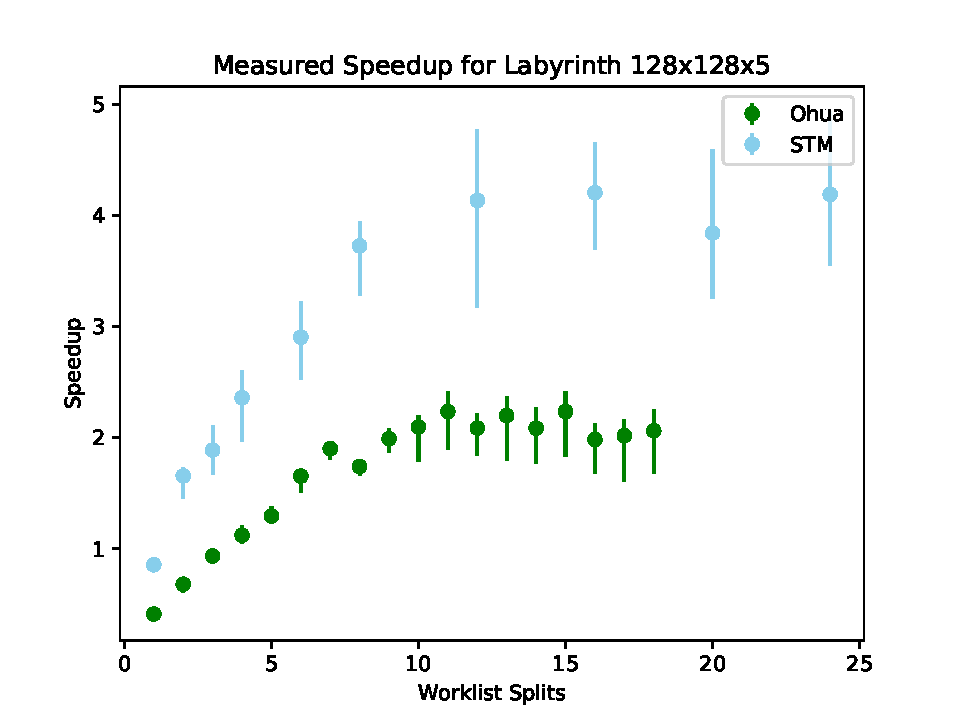
\includegraphics[width=\textwidth,height=.7\textheight,keepaspectratio]{img/split_128x128x5.pdf}}%
    \end{column}
  \end{columns}
\end{frame}

\begin{frame}{Straggler Problem with Splitting}
  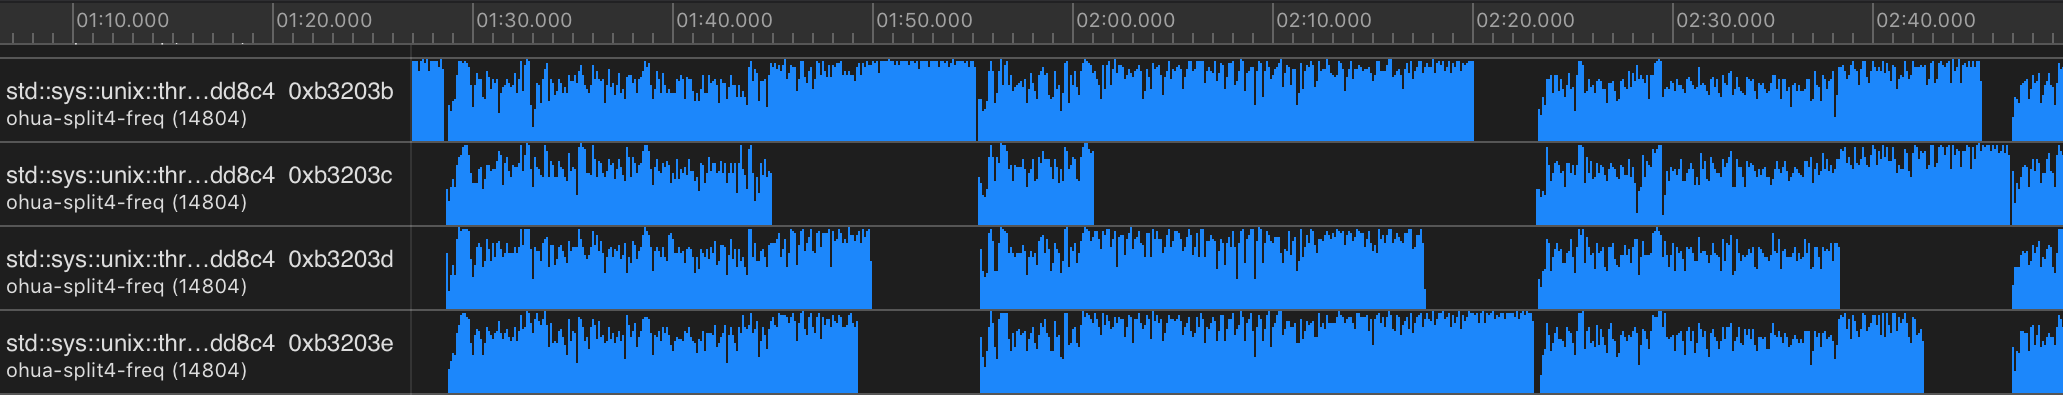
\includegraphics[width=\textwidth,keepaspectratio]{img/cpu_load_split.png}
  
  \vfill
  \begin{itemize}
    \item<2-> Worklists don't take equally long to process
    \item<3-> All threads are forced to wait at barrier
    \begin{itemize}
      \item<3-> each collision affects execution time twice
      \item<4-> uses more processing time and causes slack time for other cores
    \end{itemize}
  \end{itemize}
\end{frame}

\begin{frame}{Transformation 2: Update Frequency}
  \begin{columns}
    \begin{column}{.5\textwidth}
      \inputminted[bgcolor=rustcolor, fontsize=\tiny]{rust}{code/split.rs}
    \end{column}
    \begin{column}{.5\textwidth}
      \uncover<3->{\inputminted[bgcolor=rustcolor, fontsize=\tiny]{rust}{code/split_freq.rs}}
    \end{column}
  \end{columns}%
  \begin{itemize}
    \item<2-> Update shared state more often by only processing $n$ elements at once
  \end{itemize}
  \vfill
\end{frame}

\begin{frame}{Transformation 3: Improve Resource Utilization}
  \begin{itemize}
    \item further improve performance by utilizing work-stealing algorithms
    \item execute parallel computations on top of \texttt{tokio} framework
  \end{itemize}
\end{frame}

% TODO: Show new benchmark results (present day)
\begin{frame}{Result: Significant Performance Improvements}
  \begin{columns}
    \begin{column}{0.55\textwidth}
      \centering
      \only<1-3>{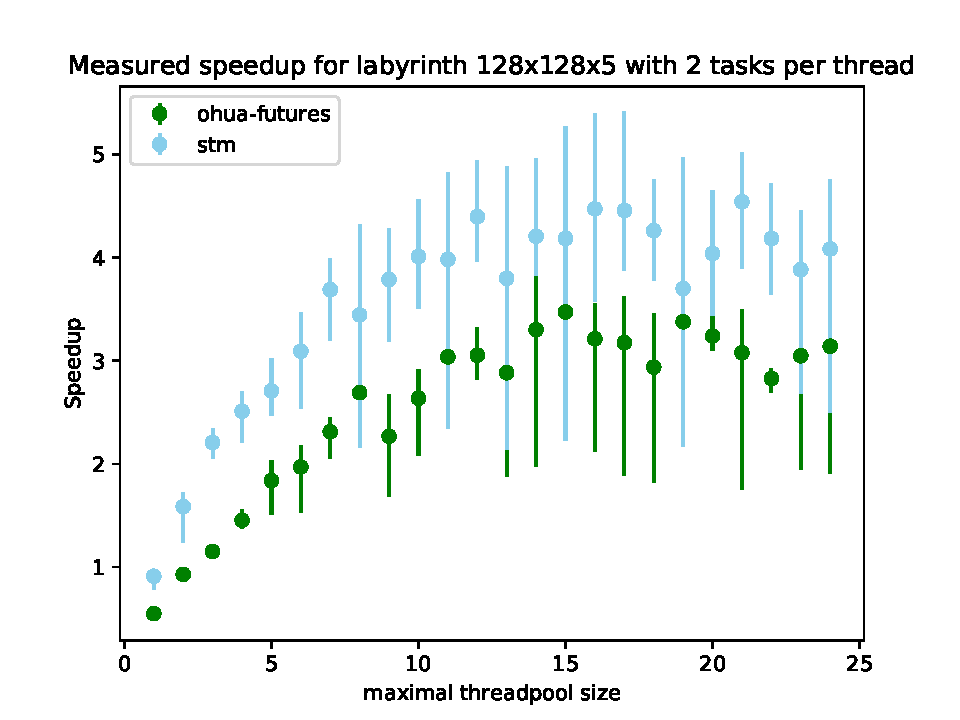
\includegraphics[width=\textwidth,height=.7\textheight,keepaspectratio]{img/current-128x128x5}}%
      \only<4->{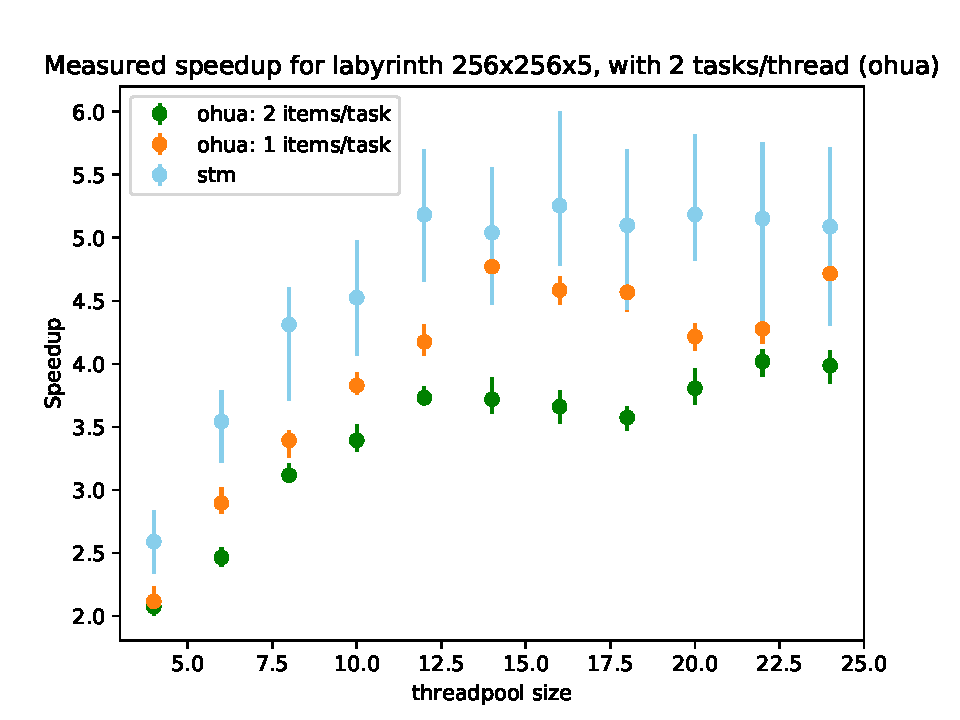
\includegraphics[width=\textwidth,height=.7\textheight,keepaspectratio]{img/futures-2tpt-256x256x5}}
    \end{column}
    \begin{column}{0.45\textwidth}
      \begin{itemize}
        \item<2-> Proof of concept: Ohua almost on par with \alert{\texttt{stm}}
        \item<3-> Advantage: deterministic execution model
        \begin{itemize}
          \item<5-> allows better debugging
          \item<6-> also reflected by execution times
        \end{itemize}
      \end{itemize}
    \end{column}
  \end{columns}
\end{frame}

\begin{frame}{Transformations: Overview}
  \textbf{General-purpose transformations applied:}\\

  \begin{enumerate}
    \item<2-> Data parallelism for stateless functions
    \begin{itemize}
      \item<2-> improve execution times\\[1.1\baselineskip]
    \end{itemize}
    \item<3-> Batch write accesses to shared state
    \begin{itemize}
      \item<3-> state updates take effect earlier\\[1.1\baselineskip]
    \end{itemize}
    \item<4-> Use work-stealing algorithm
    \begin{itemize}
      \item<4-> lessens effect of the straggler problem
    \end{itemize}
  \end{enumerate}
\end{frame}

\begin{frame}{Other benchmarks}
  \begin{itemize}
    \item According to Minh et al.\footnotemark[2] applications for \alert{\texttt{stm}} are manifold
    \item<2-> Each has own behavioral patterns\\\uncover<3->{$\rightarrow$ test Ohua on representative application range}
  \end{itemize}
  \footnotetext[2]{Minh, Chi Cao, et al. "STAMP: Stanford transactional applications for multi-processing." 2008 IEEE International Symposium on Workload Characterization. IEEE, 2008.}
\end{frame}

\begin{frame}{Benchmark 2: Intruder}
  \begin{columns}
    \begin{column}{0.55\textwidth}
      \begin{itemize}
        \item Simulates intrusion detection system
        \begin{itemize}
          \item<2-> reassembles \& inspects network packets
          \item<3-> hard to parallelize
          \item<4-> designed to show bad performance of STM\\[.55\baselineskip]
        \end{itemize}
        \item<6-> Ohua: Speedups of up to 1.25
        \item<7-> No contention due to its execution model % TODO: Is it because of the model?
      \end{itemize}
    \end{column}
    \begin{column}{0.45\textwidth}
      \uncover<5->{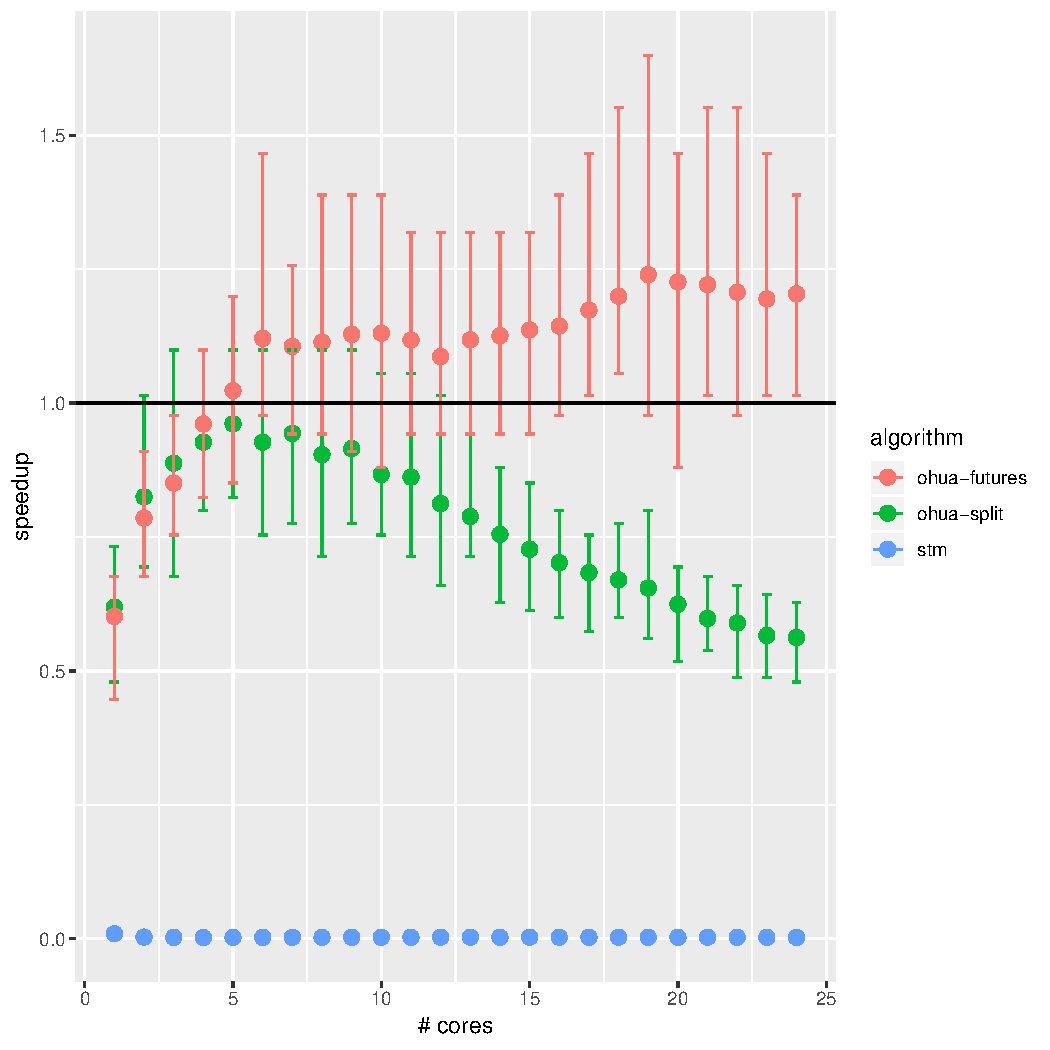
\includegraphics[width=\textwidth,height=\textheight,keepaspectratio]{img/intruder+}}
    \end{column}
  \end{columns}
\end{frame}

\begin{frame}{Next Steps}
  \begin{enumerate}
    \item Port 2-3 more benchmarks
    \begin{itemize}
      \item verify that found optimizations are applicable to other problem classes\\[1.2\baselineskip]
    \end{itemize}
    \item<2-> Implement compiler optimizations
    \begin{itemize}
      \item<2-> add dataflow transformations to the Ohua compiler\\[1.2\baselineskip]
    \end{itemize}
    \item<3-> Verify results
    \begin{itemize}
      \item<3-> using previously examined benchmarks
    \end{itemize}
  \end{enumerate}
\end{frame}

\begin{frame}
  \centering
  \huge
  \alert{\textbf{Thank you for your attention.}}
\end{frame}

% -----------------------------------------------------------------------------------------------------------
% ---------------------------------------------- BACKUP Slides ----------------------------------------------
% -----------------------------------------------------------------------------------------------------------

\begin{frame}
  \centering
  \huge
  \alert{\textbf{Backup}}
\end{frame}

\begin{frame}{Backup: Straggler Problem in STM}
  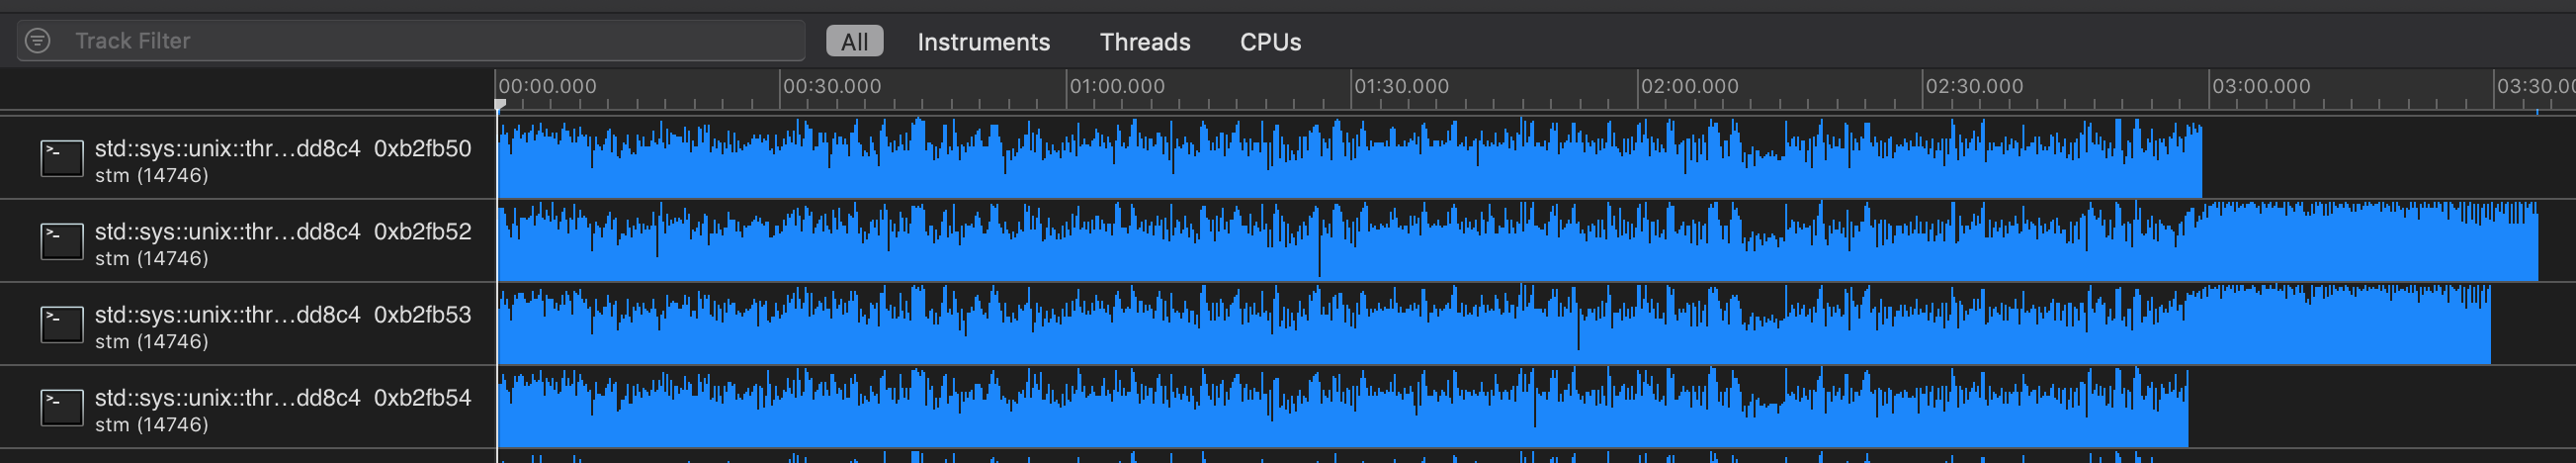
\includegraphics[width=\textwidth,keepaspectratio]{img/cpu_load_stm.png}
  
  \vfill
  \begin{itemize}
    \item<2-> STM interleaves reads and writes on shared data
    \item<3-> trade-off: no synchronization barriers \uncover<4->{but}\\[.55\baselineskip]
    \begin{itemize}
      \item<4-> non-deterministic execution model
      \item<4-> more recomputations due to state invalidation
    \end{itemize}
  \end{itemize}
\end{frame}

\begin{frame}{Backup: Benchmark Classification}
  Classification of STAMP\footnotemark[2] suite benchmarks:

  \begin{center}
    \small
    \begin{tabular}{|l|l|l|l|l|}
      \hline
      \textbf{application} & \textbf{tx length} & \textbf{r/w set} & \textbf{tx time} & \textbf{contention}\\ \hline
      labyrinth & long & large & high & high\\ \hline
bayes & long & large & high & high\\ \hline
yada & long & large & high & medium\\ \hline
vacation & medium & medium & high & low/medium\\ \hline
genome & medium & medium & high & low\\ \hline
intruder & short & medium & medium & high\\ \hline
kmeans & short & small & low & low\\ \hline
ssca2 & short & small & low & low\\ \hline
    \end{tabular}
  \end{center}

  \footnotetext[2]{Minh, Chi Cao, et al. "STAMP: Stanford transactional applications for multi-processing." 2008 IEEE International Symposium on Workload Characterization. IEEE, 2008.}
\end{frame}

\begin{frame}{Backup: Intruder Benchmark}
  \centering
  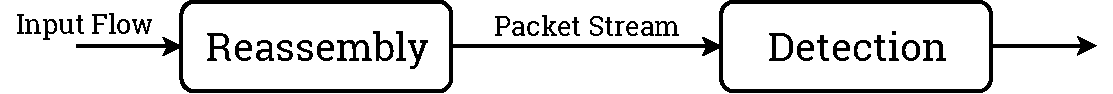
\includegraphics[width=.9\textwidth,keepaspectratio]{img/intruder-flow.pdf}
  \vspace{1cm}

  \begin{itemize}
    \item<2-> Reconstructed packets stored in shared hash map
    \item<3-> Parallel write accesses in STM provoke recomputations
  \end{itemize}
\end{frame}
% TODO: What is a "representative range" of benchmarks?

\end{document}
